\section{System Model}
    \label{sec:system_model}
    \begin{figure*}
        \centering
        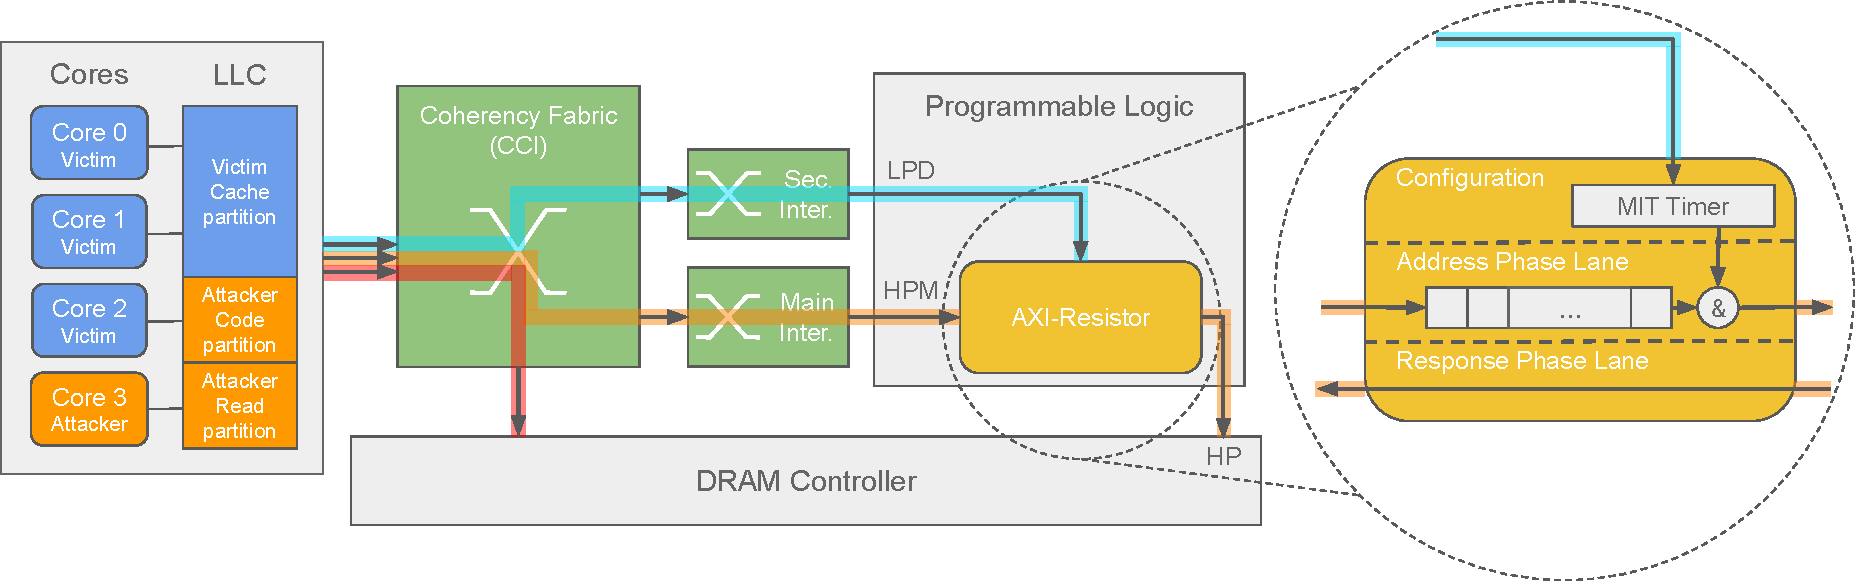
\includegraphics[scale=0.56]{images/Evaluation_setup.pdf}
        \caption{Schematic view of the considered setup with the partitioning of the core cluster (both cores and LLC) on the left, the different path taken by the transactions highlighted in purple, orange and red, and the AXI-Resistor. on the right.}
        \label{fig:system_schematic}
    \end{figure*}

    As a model, we consider a PS-PL system where the Processing System must features at least two cores and a shared non-blocking LLC.
    The PL side is programmed with a PLIM module called AXI-Resistor, which will act as a slow cacheable memory target (more details in section \ref{subsec:axi-resistor}).
    The platform resources are shared between two actors: a \emph{victim} and a \emph{attacker}.
    In the present scenario, the victim executes a set of tasks addressing directly the main memory (i.e. the path highlighted in red in Figure \ref{fig:system_schematic}), whereas the attacker mainly targets the AXI-Resistor with read transactions.
    Figure \ref{fig:system_schematic} offers a schematic representation of the platform and how it is used for the experiment.

    This section presents the details of the different components and actors of the experiment.
    Further details regarding the organization of the PS side are given in section \ref{subsec:processing_system_organization}.
    In section \ref{subsec:attacker_reading_memory_bomb}, a description of the attacker is given.
    Finally, implmentation and characteristics of the AXI-Resistor are discussed in section \ref{subsec:axi-resistor}.

    \subsection{Processing System Organization}
        \label{subsec:processing_system_organization}
        As previously mentioned, the PS side and especially the core cluster is shared by both the victim and the attacker.
        We assume a partitioned system where each actor is assigned a given set of cores and a parivate partition of the LLC.
        Consequently, each actor is independent, ensuring that the observed delays cannot be imputed to either a common software stack or inter-core cache line evictions.

        On one hand, we define our victim actor as a set of trusted applications and controllers having to meet certain deadlines.
        On the other hand, we define our attacker actor as a lightweight application in charge of emitting sequential read transactions toward the desired target.
        As shown by the Figure \ref{fig:system_schematic}, the attacker splits its private partition of the LLC in two.
        The first one half allows the attacker to access the main memory where its code is located (via the path highlighted in red in Figure \ref{fig:system_schematic}) and the second half is dedicated to the data read from AXI-Resistor (the orange path in Figure \ref{fig:system_schematic}).
        Isolating the two address space is important as it enables a high control over the amount of transactions targetting the AXI-Resistor.

        Globally, the actors are perfectly isolated.
        The only exception being that the attacker also access the main memory to fetch its code.
        Nonetheless, this should introduce little or no inter-core interference.

    \subsection{Attacker - Reading Memory Bomb}
        \label{subsec:attacker_reading_memory_bomb}
        The design of the attacker (i.e. the read memory bomb) must be thought carefully, even with the aforementioned precautions.
        In fact, if not under control a read memory bomb will steadily fetch data, creating many cache-misses.
        Following the non-blocking cache mechanism, these cache-misses will be inserted in one of the available MSHRs until all of them are used.
        In this situation the non-blocking cache controller will stop the whole machinery, leading to the phenomenon reported by \cite{Heechul_DDOS_attacks_on_shared_cache}.
        %
        This effect can only be avoided by throttling down the attacker core.
        We enforce this by following each read request by a \emph{Data Synchronisation Barrier} (\texttt{DSB}).
        This ensures that at each instant, there will not be more than one transaction in direction of the AXI-Resistor and, by extension, it guarantees that only one MSHR is occupied by the attacker actor.

    \subsection{AXI-Resistor IP}
        \label{subsec:axi-resistor}
        The AXI-resistor IP is a PLIM module \cite{PLIM20} used to act as a slow cacheable memory target in our system model.
        Typically, the IP accepts every read transaction comming from the core cluster via the HPM port, buffers them and only release them oneby one in direction of the DRAM controller after a minimal inter-arrival time (MIT) expressed in clock cycles (CC).
        This data path is highlighted in orange in Figure \ref{fig:system_schematic}.
        Because each transaction is intercepted by the the AXI-Resistor before arriving to the DRAM controller, the latter is unaware of the transaction and no internal mechanism is activated, suppressing potential interference at the level of the DRAM controller.

        The AXI-Resistor is composed of three ports: one slave port accepting transaction from the core cluster, one configuration port and one master port repeating the transactions out of the IP.
        Arriving transactions are buffered within the AXI-Resistor thanks to a queue (see \emph{Addresss Phase Lane} on the right of Figure \ref{fig:system_schematic}).
        The transaction stored at the head of the queue is released according to a rhythm dictated by a timer.
        The period of this timer is reprogrammable at run-time thanks to the configuration port.
        Once a read request has been served by the DRAM controller, the read data is sent back to the core cluster through the AXI-Resistor.
        This phase is not buffered by the IP as shown in Figure \ref{fig:system_schematic} (see \emph{Response Phase Lane}).
